
%(BEGIN_QUESTION)
% Copyright 2010, Tony R. Kuphaldt, released under the Creative Commons Attribution License (v 1.0)
% This means you may do almost anything with this work of mine, so long as you give me proper credit

Suppose we have an IEC 61131-3 compliant PLC connected to a proximity switch, a key switch, and two loads (a lamp and a solenoid coil) as shown in this illustration.  The proximity switch counts objects passing by on a conveyor belt:

$$\includegraphics[width=15.5cm]{i04528x01.eps}$$

Examine the offline display of this PLC's relay ladder logic program, determining the status of the lamp and of the solenoid coil after the proximity switch counts 6 more objects passing by, assuming the Enable keyswitch is in the ``Armed'' position and the current count value is 620.

\underbar{file i04528}
%(END_QUESTION)





%(BEGIN_ANSWER)

Both the lamp and the solenoid coil will be energized.

%(END_ANSWER)





%(BEGIN_NOTES)

With six more objects passing by, the current value will go from 620 to 626, which exceeds the counter's preset value of 624.

\vfil \eject

\noindent
{\bf Prep Quiz:}

Suppose we have an IEC 61131-3 compliant PLC connected to a proximity switch, a key switch, and two loads (a lamp and a solenoid coil) as shown in this illustration.  The proximity switch counts objects passing by on a conveyor belt:

$$\includegraphics[width=15.5cm]{i04528x01.eps}$$

Examine the offline display of this PLC's relay ladder logic program, determining the status of the lamp and of the solenoid coil after the proximity switch counts 12 more objects passing by, assuming the Enable keyswitch is in the ``Armed'' position and the current count value is 600.

%INDEX% PLC, relating I/O status to virtual elements (with counter instruction)

%(END_NOTES)


